\documentclass[12pt]{article}
\usepackage{graphicx}
\usepackage{setspace}
\usepackage[]{hyperref}
\hypersetup{backref,
			pdfpagemode=FullScreen,
			colorlinks=true,
			urlcolor=blue,
			citecolor=red}
\renewcommand{\baselinestretch}{1.2}

\begin{document}
\title{\Large Performance analysis and benchmarking of different databases for robotic applications\\
[6mm]
\Large Rubanraj Ravichandran\\
[12mm]
\Large R\&D Proposal\\
\small Master of Autonomous Systems\\
[12mm]
\Large Department of Computer Science\\
University of Applied Sciences Bonn-Rhein-Sieg\\
[12mm]
\Large Advisors:\\
Prof. Dr. Manfred Kaul\\
Nico Huebel\\
Sebastian Blumenthal
}
\date{\today}
\maketitle
\newpage
\section{Introduction}

Modern robotics applications consume and generate already lots of data. However, this will further increase with the rise of the ubiquitous sensing provided by IoT and Industry 4.0 technologies. Most of the time, perceived data from sensors has been processed for decision making and disposed after the use.
In the future, applications will require the sharing of data for the coordination of fleets of robots among themselves and with sensors in their environment. Typically, these data comes from different sources and requires different treatment. It can roughly be split into two categories:
\begin{itemize}
\item Streams of raw sensor data: This data is typically produced at high frequency and can be small (like the "tick" of an encoder) or large (like a point cloud produced by a laser scanner).
\item Metadata: This is connecting different types of sensor data together with the information and knowledge required to interpret them (like which robot has produced that data using which sensor with which settings at which position, applying which algorithm while performing what task). E.g., a point cloud of a laser scanner is not very useful if it is unknown from which position it was taken with which type of laser scanner and which settings.
\end{itemize}
As mentioned in these papers\cite{reference1}\cite{reference2}\cite{reference3}\cite{reference4}, databases used in robotics for logging system, SLAM, storing sensor data for fault analysis and performance evaluation. But, the questions are which database is fit for which task, how efficiently we can use Relational database, NoSQL\cite{reference5}, Graph database\cite{reference6}, Multi modal database for different tasks in robotics. This project focuses on qualitative analysis of a reasonable subset of currently available databases and benchmark their performance metrics under different scenarios.

\section{State of the art}
\begin{itemize}
\item A generic robot database and its application in fault analysis and performance evaluation \cite{reference1}
\begin{itemize}
\item In this paper, a well known NoSQL database Cassandra has been integrated with Robotic Operating System(ROS) to handle the data in smart environments.

\item Evaluated this approach in two scenarios,

\begin{itemize}
\item Within a realistic robot exploration
\item With a pessimistic benchmark using randomly generated data.
\end{itemize}

\item The final solution is compared with two other solutions that are commonly used in ROS applications(rosbag and mongo\_ros).

\item Advantages,
\begin{itemize}
\item Cassandra can handle terabytes of data and their timestamp mechanism allows querying and retrieving current data without additional efforts.
\end{itemize}

\item Disadvantages,
\begin{itemize}
\item ROS Cassandra implementation consumes just a bit more memory than rosbag, but even with the usage of indexes, Cassandra requires less storage than MongoDB.
\end{itemize}
\end{itemize}

\item A generic robot database and its application in fault analysis and performance evaluation\cite{reference2}
\begin{itemize}
\item In this paper, they have used highly scalable, document oriented, schema less databases MongoDB to record the data generated at run-time.

\item For this experiment, they used real domestic service robot HERB (Home Exploring Robot Butler) which produces huge among of data about 120MB/min and at peak rates of 500MB/min.

\item For performance benchmarking RRD(Round Robin Database) tool has been used to analyse the CPU and memory utilization.

\item Advantages,
\begin{itemize}
\item This approach will be helpful for fault analysis and peformance evaliuation between fleet of robots.
\end{itemize}
\end{itemize}

\item Benchmarking of Relational and NoSQL Databases to Determine Constraints for Querying Robot Execution Logs\cite{reference3},

\begin{itemize}
\item In this projectan extensive benchmarking study has been conducted to find which database performs well for the ROS(Robot Operating System).

\item The main focus of this study is to subsume the use of rosbags and instead integrate databases to collect and analyze logs for future use. For experiment, MongoDB, PostgreSQL, SQLite3 databases examined based on number of messages, the size of messages and the number of topics.

\item Advantages,
\begin{itemize}
\item This approach proved that, MongoDB is the best fit for handling ROS logs.
\item Compared maximum throughput for both synthetic and real-world datasets.
\end{itemize}

\item Disadvantages,
\begin{itemize}
\item Specific data querying option is not available in rosbags.
\item PostgreSQL and SQLite3 throughput is minimum compared to MongoDB and this databases is difficult to adapt dynamic changes in data model.
\end{itemize}
\end{itemize}
\newpage

\item SLAMinDB: Centralized graph databases for mobile robotics\cite{reference4}

\begin{itemize}
\item This paper demonstrates the use of centralized factor-graph for data persistence.

\item Graph data model and key value pair model is used to represent the data generated by robot application. Large size data are stored in MongoDB and the key reference is given to Neo4J graph database.
\item Advantages,
\begin{itemize}
\item Graph database handles the relationship between the data generated and it stores the tiny data like odometric values.

\item Using centralized graph database is helpful for sharing data, especia6ioully in terms of cooperative agents.
\end{itemize}
\end{itemize}

\item Conclusion:
\begin{itemize}
\item From all this approaches discussed above, they focused on very specific applications/settings and are always comparing only very few databases within this limited setting. Moreover, they benchmarked the performance with single robot in most of the cases. This benchmarking may not be helpful in multiple robot scenarios. Our intention of this work is, to go beyond that by comparing different model databases in multiple settings/robots. \cite{reference4} seems to go in the direction of what we expect to be the best solution (combination of graph + data storage) and we will be further explored.
\end{itemize}
\end{itemize}

\section{Problem formulation}

The problem addressed in this work is, there is no specific databases available in the market for robotic applications and our task is to identify a set of databases and benchmark them to decide which database will be fit for robotic applications.

When data about different robots and their environment is combined this is called a world model. These days, developers in robotics often use self-written, ad-hoc solutions for handling robotic data. However, in recent years many commercial as well as open-source databases became available that perform similar tasks while promising better performance (wrt features, performance, and querying) as well as additional features compared to the ad-hoc solutions from robotics. However, they all come with advantages and disadvantages and were not designed for robotic applications. So the robotic specific structures and data models need to be imposed on these databases.
\\

\section{Approach}
To address this problem, set of Relational, NoSQL, Graph and multi-model databases will be compared qualitatively based on their features. For comparison, databases will be collected from state-of-the-art techniques and current top ranked databases. The selected features will take common DB criterias into account. Furthermore, features will be derived from the below robotic usecases. Benchmarking scenarios will be defined and implemented from robotic research project(e.g. ROPOD). Setting up the selection of databases in the docker container for benchmarking. Finally, a selection of the databases will be compared against the benchmarking scenarios. This comparison is based on the performance evaluation metrics(e.g. throughput, query execution time, message size, frequency and number of robots involved in the scene). The result will be a suggestion for the best practice when to use which database in robotics.

\newpage
\subsection{Robotic usecases}
\begin{itemize}
  \item Robots streaming sensor data:
  \begin{itemize}
    \item Number of robots: 1, 10, 100, 1000, 10000 robots.
    \item Size of data packages: simple floats, structs containing floats + strings, image streams (binary), binary data (relatively large) + metadata.
    \item Frequency of sending.
    \begin{itemize}
    		\item Bandwidth limitations (e.g. WIFI dropouts)
    \end{itemize}
  \end{itemize}
\end{itemize}
\begin{itemize}
  \item Querying
  \begin{itemize}
    \item Querying of attributes (e.g. give me the battery level of that robot)
    \item Querying of attribute and history (e.g. give me pose of that robot over the last 10 sec)
    \item Querying of structures (sub-graphs or tables; e.g. give me all information from a certain area)
    \item Dialogues (iteratively refining queries; e.g. give me the semantic map of that floor, now give me all rooms that contain a certain attribute like a charging station)
    \item Cursors (e.g. give me the last 100 sensor readings, now give me the next 100)
  \end{itemize}
\end{itemize}
\begin{itemize}
\item Processing
\begin{itemize}
\item Compacting and logging stream to file/other table/...
\item Run filter on history of data and create new data (e.g. filtering or fusing sensor data)
\end{itemize}
\end{itemize}
\newpage

\section{Workplan}
This workplan shows the major decomposition of the workpackages, start time and end time. This project starts on June 1, 2017 for 8 months duration and ends on January 15,2018.
\subsection{Work packages}
\begin{figure}[h!]
  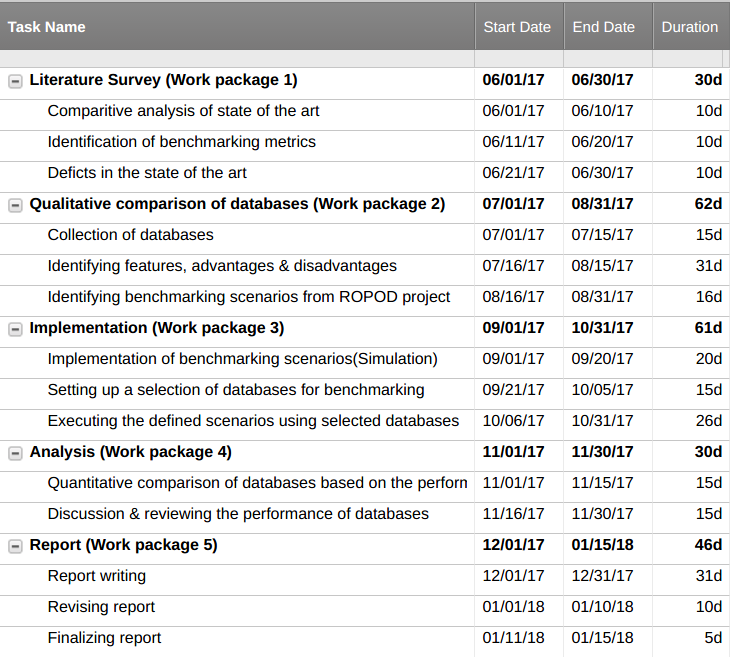
\includegraphics[width=\linewidth]{work_packages.png}
  \caption{Work packages}
  \label{fig:work_packages}
\end{figure}
\newpage
\subsection{Gantt Chart}
\begin{figure}[h!]
  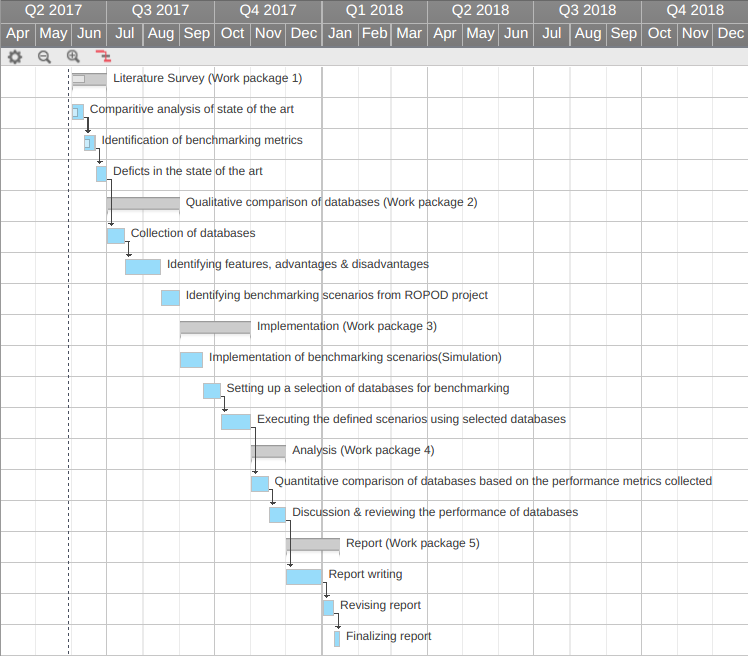
\includegraphics[width=\linewidth]{gantt_chart.png}
  \caption{Gantt Chart}
  \label{fig:gantt_chart}
\end{figure}
\newpage
\section{Deliverables}
\subsection{Minimum}
\begin{itemize}
\item Comparative analysis report on state of the art.
\item Collection of different model databases.
\item Qualitative comparison of databases based on features, advantages and disadvantages.
\end{itemize}
\subsection{Expected}
\begin{itemize}
\item Benchmarking scenarios setup in simulation and database setup.
\item Quantitative analysis on a selection of databases against defined scenarios.
\end{itemize}
\subsection{Maximum}
\begin{itemize}
\item A report describing benchmark scenarios in robotics and which DB is most suitable for which scenario.
\end{itemize}

\section{References}
\begin{thebibliography}{9}
\bibitem{reference1}
T. Niemueller, G. Lakemeyer and S. S. Srinivasa, ”A generic robot database and its application in fault analysis and performance evaluation,” 2012 IEEE/RSJ International Conference on Intelligent Robots and Systems, Vilamoura, 2012, pp. 364-369.
\bibitem{reference2}
Dietrich, André, et al. "Ros meets cassandra: Data management in smart environments with nosql." Proc. of the 11th Intl. Baltic Conference (Baltic DB\&IS). 2014.
\bibitem{reference3}
Fiannaca, Alexander J., and Justin Huang. "Benchmarking of Relational and NoSQL Databases to Determine Constraints for Querying Robot Execution Logs." Computer Science \& Engineering, University of Washington, USA (2015): 1-8.
\bibitem{reference4}
SLAMinDB: Centralized graph databases for mobile robotics
D. Fourie, S. Claassens, S. Pillai, R. Mata, J. Leonard
International Conference on Robotics and Automation (ICRA), 2017 (Not published yet, Ref: \href{https://people.csail.mit.edu/spillai/projects/cloud-graphs/}{https://people.csail.mit.edu/spillai/projects/cloud-graphs/})
\bibitem{reference5}
R. Hecht and S. Jablonski, "NoSQL evaluation: A use case oriented survey," 2011 International Conference on Cloud and Service Computing, Hong Kong, 2011, pp. 336-341.
\bibitem{reference6}
Angles, Renzo. "A comparison of current graph database models." Data Engineering Workshops (ICDEW), 2012 IEEE 28th International Conference on. IEEE, 2012.
\end{thebibliography}
\end{document}
